\documentclass[a4paper,11pt,twocolumn]{article}
\usepackage{fancyhdr}
\usepackage{enumerate}
\usepackage{times}
\usepackage{mathptmx}
\usepackage{amsmath}
\usepackage{amsfonts}
\usepackage{amssymb}
\usepackage{tikz}
\usepackage{graphicx}
\usepackage[top=2cm, bottom=2cm, left=2cm, right=2cm]{geometry}

\setlength{\columnsep}{7mm}

\newcommand{\homeworkno}{3.6}
\pagestyle{fancy}
\lhead{Problem Solving: Homework \homeworkno}
\chead{}
\rhead{Chen Shaoyuan (161240004)}
\lfoot{}
\cfoot{\thepage}
\rfoot{}

\allowdisplaybreaks[4]
\renewcommand{\labelenumi}{(\alph{enumi})}
\begin{document}
  \title{Problem Solving: Homework \homeworkno}
  \author{Name: Chen Shaoyuan \and Student ID: 161240004}
  \maketitle

  \section{[GC] Problem 8.1}
  \begin{enumerate}
    \item $G$:
    \small
    \begin{center}
    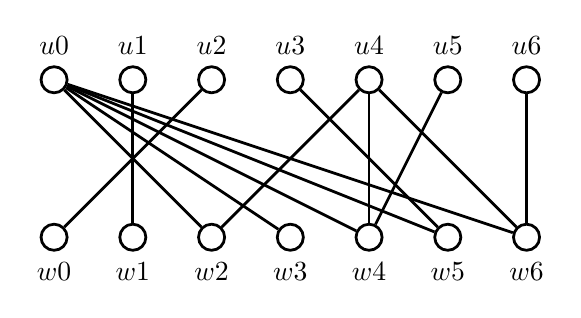
\begin{tikzpicture}[line width = 1pt,
                        solid/.style = {circle, draw, fill = black, minimum size = 0.1cm},
                        empty/.style = {circle, draw, fill = white, minimum size = 0.1cm}]
      \node [empty, label={above:$u0$}] (u0) at (0, 2){};
      \node [empty, label={above:$u1$}] (u1) at (1, 2){};
      \node [empty, label={above:$u2$}] (u2) at (2, 2){};
      \node [empty, label={above:$u3$}] (u3) at (3, 2){};
      \node [empty, label={above:$u4$}] (u4) at (4, 2){};
      \node [empty, label={above:$u5$}] (u5) at (5, 2){};
      \node [empty, label={above:$u6$}] (u6) at (6, 2){};
      \node [empty, label={below:$w0$}] (w0) at (0, 0){};
      \node [empty, label={below:$w1$}] (w1) at (1, 0){};
      \node [empty, label={below:$w2$}] (w2) at (2, 0){};
      \node [empty, label={below:$w3$}] (w3) at (3, 0){};
      \node [empty, label={below:$w4$}] (w4) at (4, 0){};
      \node [empty, label={below:$w5$}] (w5) at (5, 0){};
      \node [empty, label={below:$w6$}] (w6) at (6, 0){};
      \draw (u0) -- (w2); \draw (u0) -- (w3); \draw (u0) -- (w4); \draw (u0) -- (w5); \draw (u0) -- (w6);
      \draw (u1) -- (w1);
      \draw (u2) -- (w0);
      \draw (u3) -- (w5);
      \draw (u4) -- (w2); \draw (u4) -- (w4); \draw (u4) -- (w6);
      \draw (u5) -- (w4);
      \draw (u6) -- (w6);
    \end{tikzpicture}
    \end{center} \par
    \normalsize
    \item Yes. A perfect matching is
    \small
    \begin{center}
    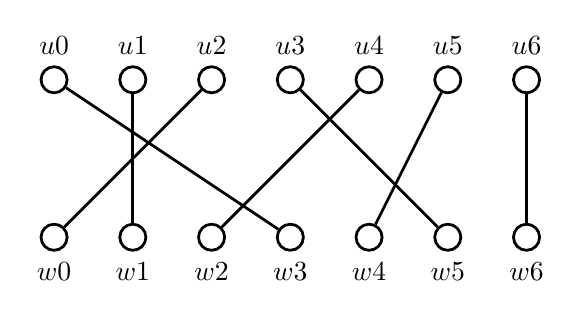
\begin{tikzpicture}[line width = 1pt,
                        solid/.style = {circle, draw, fill = black, minimum size = 0.1cm},
                        empty/.style = {circle, draw, fill = white, minimum size = 0.1cm}]
      \node [empty, label={above:$u0$}] (u0) at (0, 2){};
      \node [empty, label={above:$u1$}] (u1) at (1, 2){};
      \node [empty, label={above:$u2$}] (u2) at (2, 2){};
      \node [empty, label={above:$u3$}] (u3) at (3, 2){};
      \node [empty, label={above:$u4$}] (u4) at (4, 2){};
      \node [empty, label={above:$u5$}] (u5) at (5, 2){};
      \node [empty, label={above:$u6$}] (u6) at (6, 2){};
      \node [empty, label={below:$w0$}] (w0) at (0, 0){};
      \node [empty, label={below:$w1$}] (w1) at (1, 0){};
      \node [empty, label={below:$w2$}] (w2) at (2, 0){};
      \node [empty, label={below:$w3$}] (w3) at (3, 0){};
      \node [empty, label={below:$w4$}] (w4) at (4, 0){};
      \node [empty, label={below:$w5$}] (w5) at (5, 0){};
      \node [empty, label={below:$w6$}] (w6) at (6, 0){};
      \draw (u0) -- (w3);
      \draw (u1) -- (w1);
      \draw (u2) -- (w0);
      \draw (u3) -- (w5);
      \draw (u4) -- (w2);
      \draw (u5) -- (w4);
      \draw (u6) -- (w6);
    \end{tikzpicture}
    \end{center} \par
    \normalsize
    This means that there exists a permutation $\pi$ of $\{0, 1, 2, 3, 4, 5, 6\}$, such that $w_{\pi(i)}$ is a correct response to $u_i$, for $0 \leq i \leq 6$.
  \end{enumerate}

  \section{[GC] Problem 8.3}
  For graph $G_1$, $U$ can be matched to $W$. One possible matching is $\{(a, x), (b, w), (c, v), (d, z), (e, y)\}$. \par
  For graph $G_2$, $U$ can't be matched to $W$. Consider vertex set $\{b, d, e\}$, the cardinality of its neighborhood is only 2, which violates Hall's condition.

  \section{[GC] Problem 8.4}
  For all subset $U'$ of $U$, since every two vertices in $U'$ have distinct degrees, the maximum degree of all vertices of $U'$ is at least $|U'|$, and thus the cardinality of the neighborhood of $U'$ is at least $|U'|$. Therefore, the graph $G$ satisfies Hall's condition, which means $G$ contains a perfect matching.

  \section{[GC] Problem 9.6}
  \begin{enumerate}
    \item True. It is obvious that if a graph does not contain a subdivision of $K_5$ or $K_{3,3}$, neither does its subgraph. Therefore, by Kuratowski's Theorem, every subgraph of a planar graph is planar.
    \item False. For any nonplanar graph, if we take one of its vertices as a trivial subgraph, then it is obviously a planar subgraph.
    \item False. Consider $K_5$, removing any of its edges or vertices will make the resulting graph not contain a subdivision of $K_5$ or $K_{3,3}$, so $K_5$ is a counterexample to this statement.
    \item False. If we insert an vertex to any edge of $K_5$, the resulting graph does not contain $K_5$ or $K_{3,3}$ as a subgraph, however, it is still nonplanar.
    \item False. Consider the union of $K_5$ and $C_3$, with order $n = 8$ and size $m = 13$, which satisfies $m \leq 3n-6$. However, one of its components is nonplanar, and thus the graph is nonplanar.
    \item False. Consider the union of $K_{3,3}$ and $C_3$, it has a triangle and contains no subdivision of $K_5$ as a subgraph, however, it is  nonplanar.
  \end{enumerate}
  
  \section{[GC] Problem 9.13}
  \begin{enumerate}
    \item Since $G$ contains no triangle, the boundary of every region has at least 4 edges. Because every edge belongs to at most two of the boundaries, we have $2m \geq 4r$, i.e. $2r \leq m$. By Euler's Identity, we have $r=2+m-n$. Hence, $4+2m-2n \leq m$, i.e. $m \leq 2n-4$.
    \item For $K_{3,3}$, $n = 6$, $m = 9$, $m > 2n - 4$. Note that $K_{3,3}$ contains no triangle, so $K_{3,3}$ is nonplanar.
    \item This is true. First, $G$ contains no triangle because it is bipartite. Suppose that every vertex has degree 4 or more, then $2m \geq 4n$, i.e. $m \geq 2n$, which violates the inequality we proved in (a). Therefore, $G$ has a vertex of degree 3 or less.
  \end{enumerate}
  
  \section{[GC] Problem 9.14}
  \begin{enumerate}
    \item Since the length of a smallest cycle in $G$ is 5, the boundary of every region has at least 5 edges. Because every edge belongs to at most two of the boundaries, we have $2m \geq 5r$. By Euler's Identity, we have $r=2+m-n$. Hence $2+m-n\leq\frac{2}{5}m$, i.e. $m \leq \frac{5}{3}(n-2)$.
    \item Petersen graph has 15 edges and 10 vertices, so $m > \frac{5}{3}(n-2)$. Since the length of a smallest cycle in Petersen graph is 5, it is nonplanar.
    \item Removing any vertex of the Petersen graph yields a subdivision of $K_{3,3}$, so the Peterson graph is nonplanar.
    \begin{figure}[h]
        \centering
        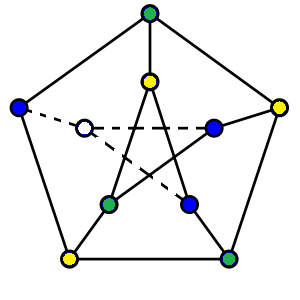
\includegraphics{petersen_nonplanar.png}\\
    \end{figure}
    \item Suppose, to the contrary that every vertex of $G$ has a degree of 3 or more, then $2m \geq 3n$. Therefore, $\frac{3}{2}n \leq m \leq \frac{5}{3}(n-2)$. After some algebra we get $n \geq 20$, which leads to contradiction.
  \end{enumerate}
\end{document}
